\clearpage
\section{Chapter four}

% %%%%%%%%%%%%%%%%%%%%%%%%%%%%%%%%%%%%%%%%%%%%%%%%%%%%%%%
%
% %%%%%%%%%%%%%         SECTION 3          %%%%%%%%%%%%%%
%
% %%%%%%%%%%%%%%%%%%%%%%%%%%%%%%%%%%%%%%%%%%%%%%%%%%%%%%%

\vspace*{\fill}

\begin{example}
  \centering
  \includegraphics[width=\linewidth]{c/3/ex/lussy-mattheson.png}
  \caption{Mattheson, Minuet parsed using punctuation, 1739}
  \label{mus:mattheson}
\end{example}

\vspace*{\fill}

\begin{example}
  \centering
  \includegraphics[width=\linewidth]{c/3/ex/gevaert_dots.jpg}
  \caption{Gevaert, Dotted annotations, 1875}
  \label{mus:gevaert_dots}
\end{example}

\vspace*{\fill}

\begin{example}
  \centering
  \includegraphics[width=\linewidth]{c/3/ex/marcetteau_beethoven.png}
  \caption{Marcetteau, Dots showing metrical accents, 1909}
  \label{mus:marcetteau-dots}
\end{example}

\newpage

\vspace*{\fill}

\begin{example}
  \centering
  \includegraphics[width=.4\linewidth]{c/3/ex/wagner_majorcadence.png}
  \caption{Wagner, Niedermeyan cadence, 1895}
  \label{mus:wagner_majorcadence}
\end{example}

\vspace*{\fill}

\begin{example}
  \centering
  \includegraphics[width=.4\linewidth]{c/3/ex/wagner_minorcadence.png}
  \caption{Wagner, Flatted V--I cadence, 1895}
  \label{mus:wagner_minorcadence}
\end{example}

\vspace*{\fill}

\begin{example}
  \centering
  \includegraphics[width=.6\linewidth]{c/3/ex/moc_punct_128.png}
  \caption{Mocquereau, Pointing \emph{arsic} and \emph{thetic} \emph{ictuses}, 1897}
  \label{mus:moc_punctuation}
\end{example}

\vspace*{\fill}

\newpage

\vspace*{\fill}

\begin{example}
  \centering
  \includegraphics[width=\linewidth]{c/3/ex/delpech_asperges_1.jpg}
  \caption{Mocquereau-Delpech, Pointed `Asperges me', 1898}
  \label{mus:delpech_asperges_1}
\end{example}

\vspace*{\fill}

\newpage

\vspace*{\fill}

\begin{example}
  \centering
  \includegraphics[width=\linewidth]{c/3/ex/delpech_caret_47.png}
  \caption{\emph{Pressus} attracting primary \emph{arsic} \emph{ictus}, 1898}
  \label{mus:delpech_caret_47}
\end{example}

\vspace*{\fill}

\begin{example}
  \centering
  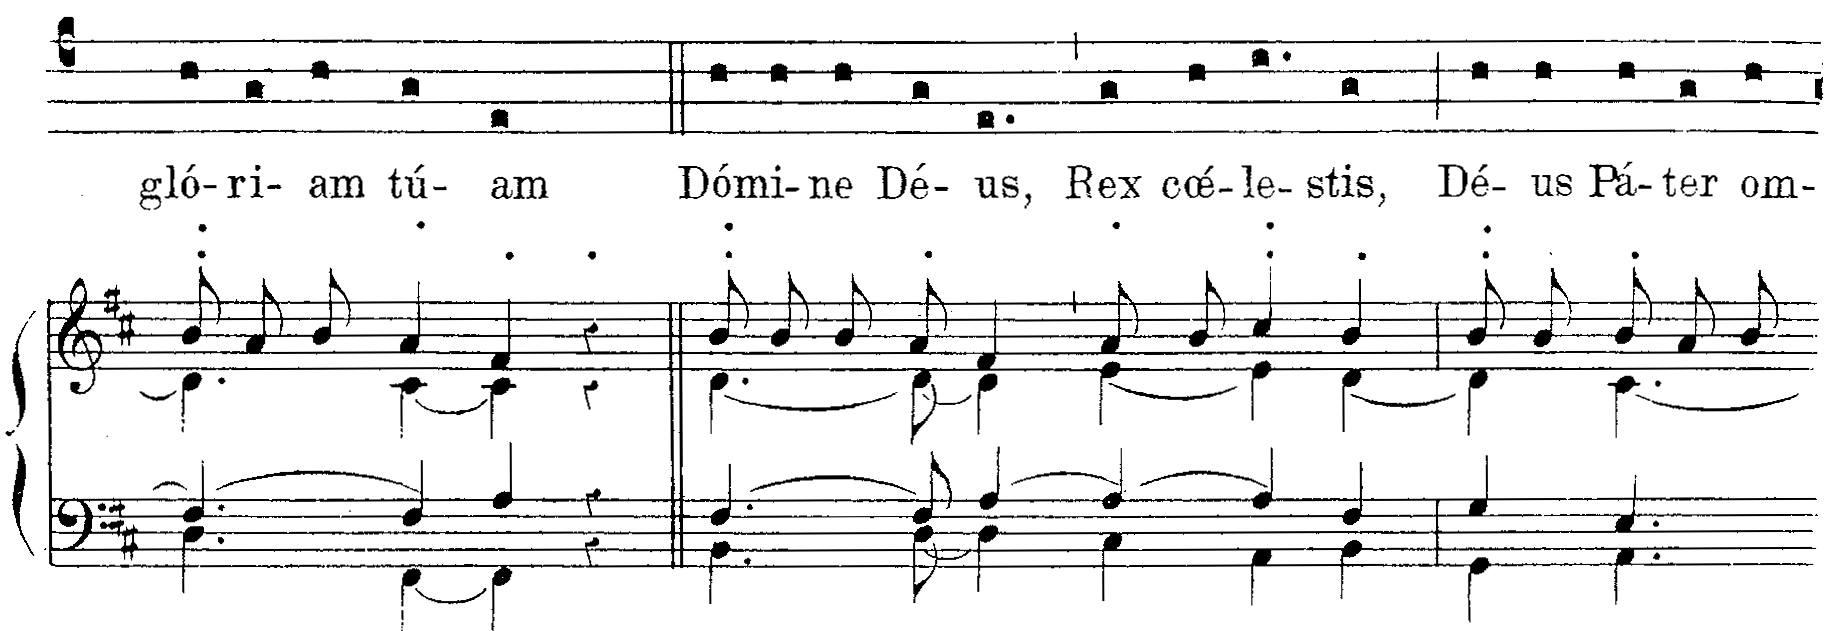
\includegraphics[width=\linewidth]{c/3/ex/delpech_livre_2_87.png}
  \caption{\emph{Mora vocis} attracting primary \emph{arsic} \emph{ictus}, 1898}
  \label{mus:delpech_livre_2_87}
\end{example}

\vspace*{\fill}

\begin{landscape}

 \vspace*{\fill}

  \begin{example}
    \centering
    \includegraphics[width=.8\linewidth]{c/3/ex/legeay_4_14.png}
    \caption{Legeay, Beamed notation, 1892}
    \label{mus:legeay_4_14}
  \end{example}

  \vspace*{\fill}

\end{landscape}

\vspace*{\fill}

\begin{example}
  \centering
  \includegraphics[width=\linewidth]{c/3/ex/lepage_85.jpg}
  \caption{Lepage, \ldo{} notation, 1900}
  \label{mus:lepage_85}
\end{example}

\vspace*{\fill}

\begin{example}
  \centering
  \includegraphics[width=\linewidth]{c/3/ex/delpech_deuterus_23.png}
  \caption{Delpech, 5/3 chords built on \pitch{6} in the deuterus, 1898}
  \label{mus:delpech_deuterus_23}
\end{example}

\vspace*{\fill}

\newpage

\vspace*{\fill}

\begin{example}
  \centering
  \includegraphics[width=.6\linewidth]{c/3/ex/latombelle_pascha.png}
  \caption{Mocquereau--La Tombelle, Chord placement follows pointing, 1898}
  \label{mus:latombelle_pascha}
\end{example}

\vspace*{\fill}

\begin{example}
  \centering
  \includegraphics[width=.9\linewidth]{c/3/ex/guilmant_haec.png}
  \caption{Mocquereau--Guilmant, Independence from primary \emph{arsic} \emph{ictus}, 1898}
  \label{mus:guilmant_haec}
\end{example}

\vspace*{\fill}

\newpage

\vspace*{\fill}

\begin{example}
  \centering
  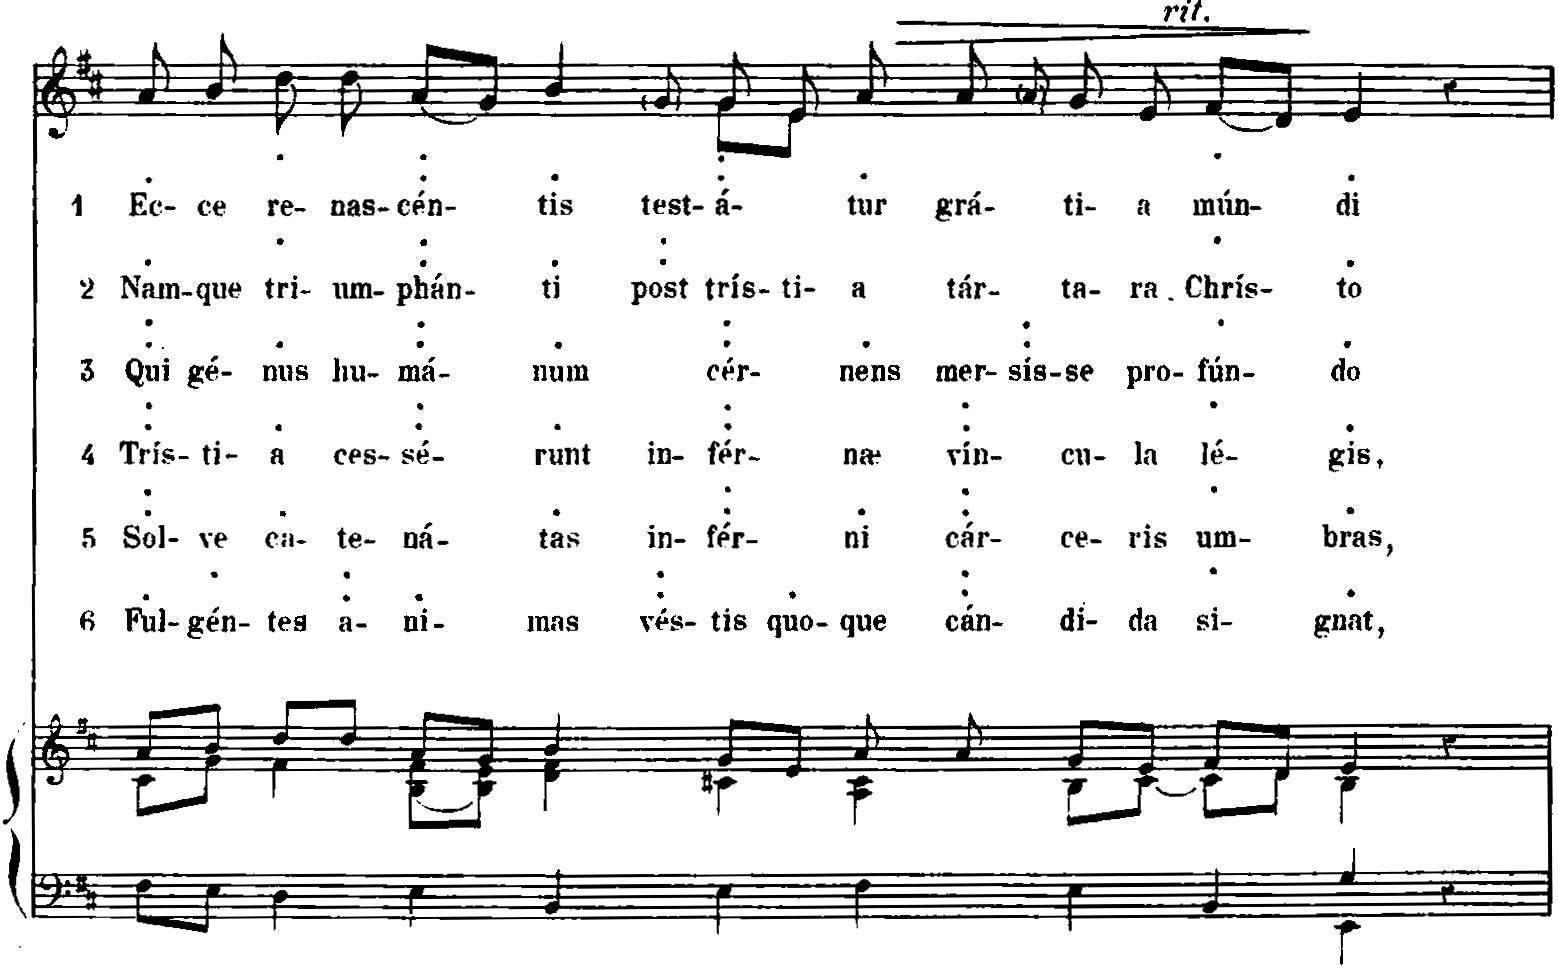
\includegraphics[width=.9\linewidth]{c/3/ex/bordes_salvefesta_10.png}
  \caption{Mocquereau--Bordes, Each verse pointed, 1898}
  \label{mus:bordes_salvefesta_10}
\end{example}

\vspace*{\fill}

\begin{example}
  \centering
  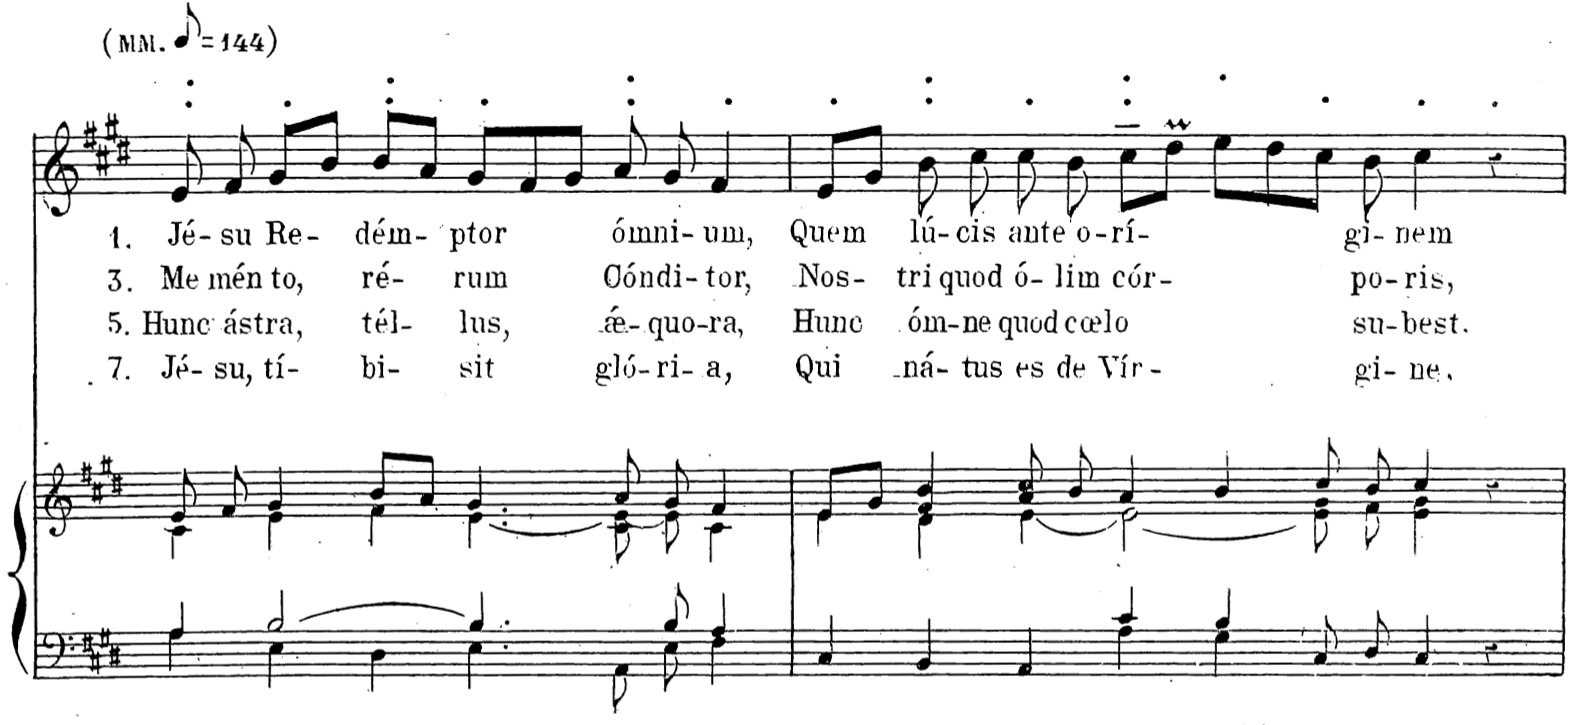
\includegraphics[width=\linewidth]{c/3/ex/guilmant_jesuredemptor.png}
  \caption{Mocquereau--Guilmant, Chant pointed instead of text, 1898}
  \label{mus:guilmant_jesu}
\end{example}

\vspace*{\fill}

\newpage

\vspace*{\fill}

\begin{example}
  \centering
  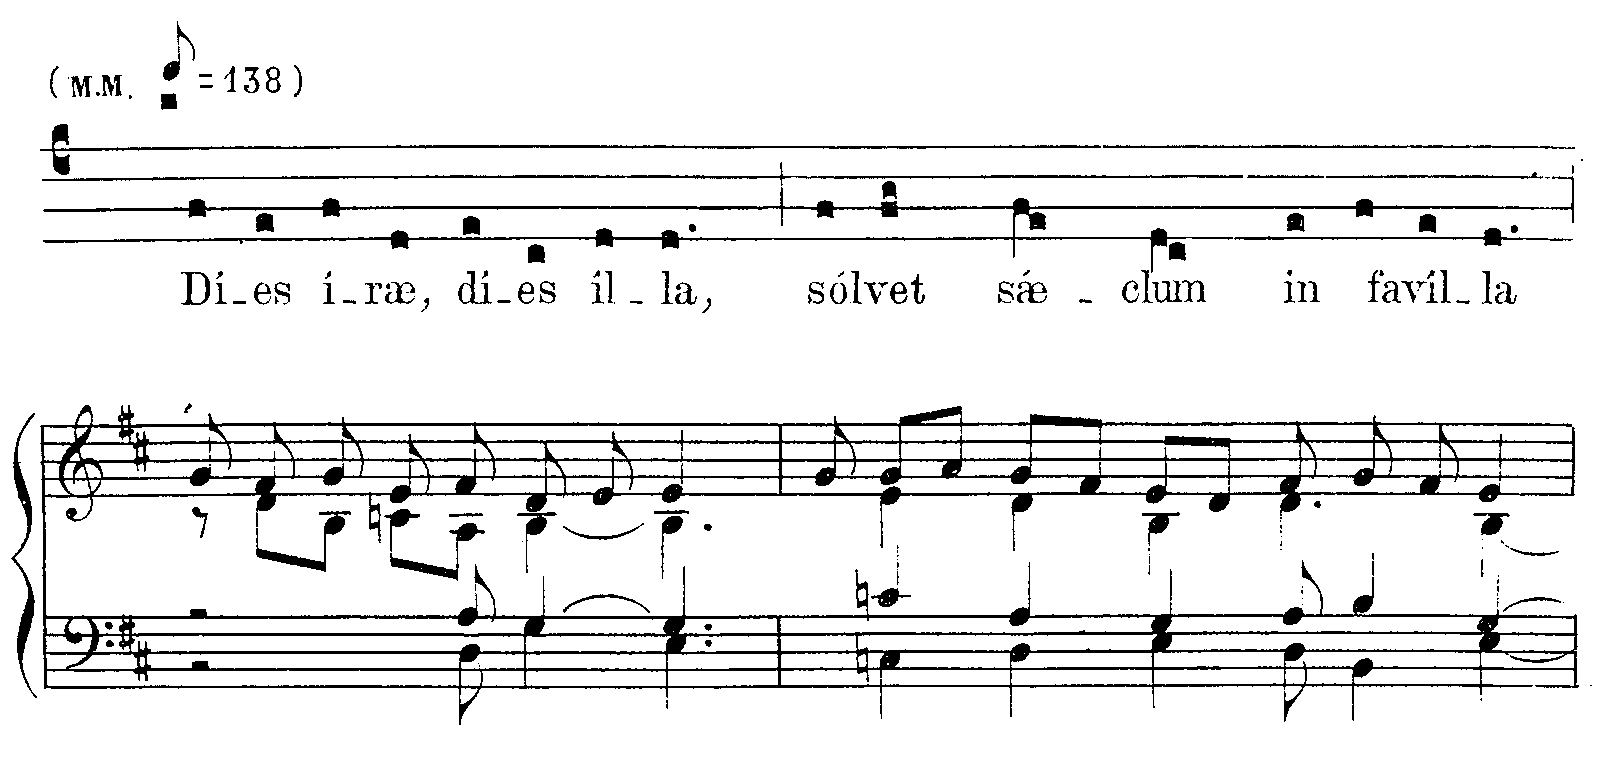
\includegraphics[width=.9\linewidth]{c/3/ex/livre_diesirae.png}
  \caption{Mocquereau--Delpech, Chords change on unaccented syllables, 1900}
  \label{mus:livre_diesirae_142}
\end{example}

\vspace*{\fill}

\begin{example}
  \centering
  \includegraphics[width=.8\linewidth]{c/4/ex/bas_gaborit_19.png}
  \caption{Gaborit analysing Bas, 1903}
  \label{mus:bas_gaborit_19}
\end{example}

\vspace*{\fill}

\newpage

\vspace*{\fill}

\begin{example}
  \centering
  \includegraphics[width=.4\linewidth]{c/4/ex/bas_allsaints.png}
  \caption{Bas, Supposedly syncopated chord placement, 1903}
  \label{mus:bas_allsaints}
\end{example}

\vspace*{\fill}

\begin{example}
  \centering
  \includegraphics[width=.5\linewidth]{c/4/ex/laloy_dominum.png}
  \caption{Laloy, Alternative transcription, 1903}
  \label{mus:laloy_dominum}
\end{example}

\vspace*{\fill}

\begin{example}
  \centering
  \includegraphics[width=.9\linewidth]{c/4/ex/solesmes_pointing_26.png}
  \caption{Solesmes, New method of pointing \emph{ictuses}, 1904}
  \label{mus:solesmes_pointing_26}
\end{example}

\vspace*{\fill}

\newpage

\vspace*{\fill}

\begin{example}
  \centering
  \includegraphics[width=\linewidth]{c/4/ex/bas_salve.png}
  \caption{Bas, Chord placement on weak syllables, 1903}
  \label{mus:bas_salve}
\end{example}

\vspace*{\fill}

\newpage

\vspace*{\fill}

\begin{example}
  \centering
  \includegraphics[width=.5\linewidth]{c/4/ex/bas_gaborit.jpg}
  \caption{Bas, Incorporating Gaborit's correction, \emph{c}.1904}
  \label{mus:bas_gaborit}
\end{example}

\vspace*{\fill}

\begin{example}
  \centering
  \includegraphics[width=.8\linewidth]{c/4/ex/bas_laloy.jpg}
  \caption{Bas, Incorporating Laloy's correction, \emph{c}.1904}
  \label{mus:bas_laloy}
\end{example}

\vspace*{\fill}

\begin{example}
  \centering
  \includegraphics[width=.7\linewidth]{c/4/ex/bas_bewerungecritic.jpg}
  \caption{Bas, Extract from `In Epiphania Domini'}
  \label{mus:bas_bewerungecritic}
\end{example}

\vspace*{\fill}

\newpage

\vspace*{\fill}


\begin{example}
  \centering
  \includegraphics[width=.9\linewidth]{c/4/ex/bas_epiphany_4.JPG}
  \caption{Bas, Rests in the accompaniment, 1904}
  \label{mus:bas_epiphany_4}
\end{example}

\vspace*{\fill}

\begin{example}
  \centering
  \includegraphics[width=\linewidth]{c/4/ex/bas_paleo.jpg}
  \caption{Bas, Determining treatment of the \emph{ictus}, \emph{c}.1905}
  \label{mus:bas_paleo}
\end{example}

\vspace*{\fill}

\newpage

\vspace*{\fill}

\begin{example}
  \centering
  \includegraphics[width=.75\linewidth]{c/4/ex/mathias_graduated_1.png}\\
  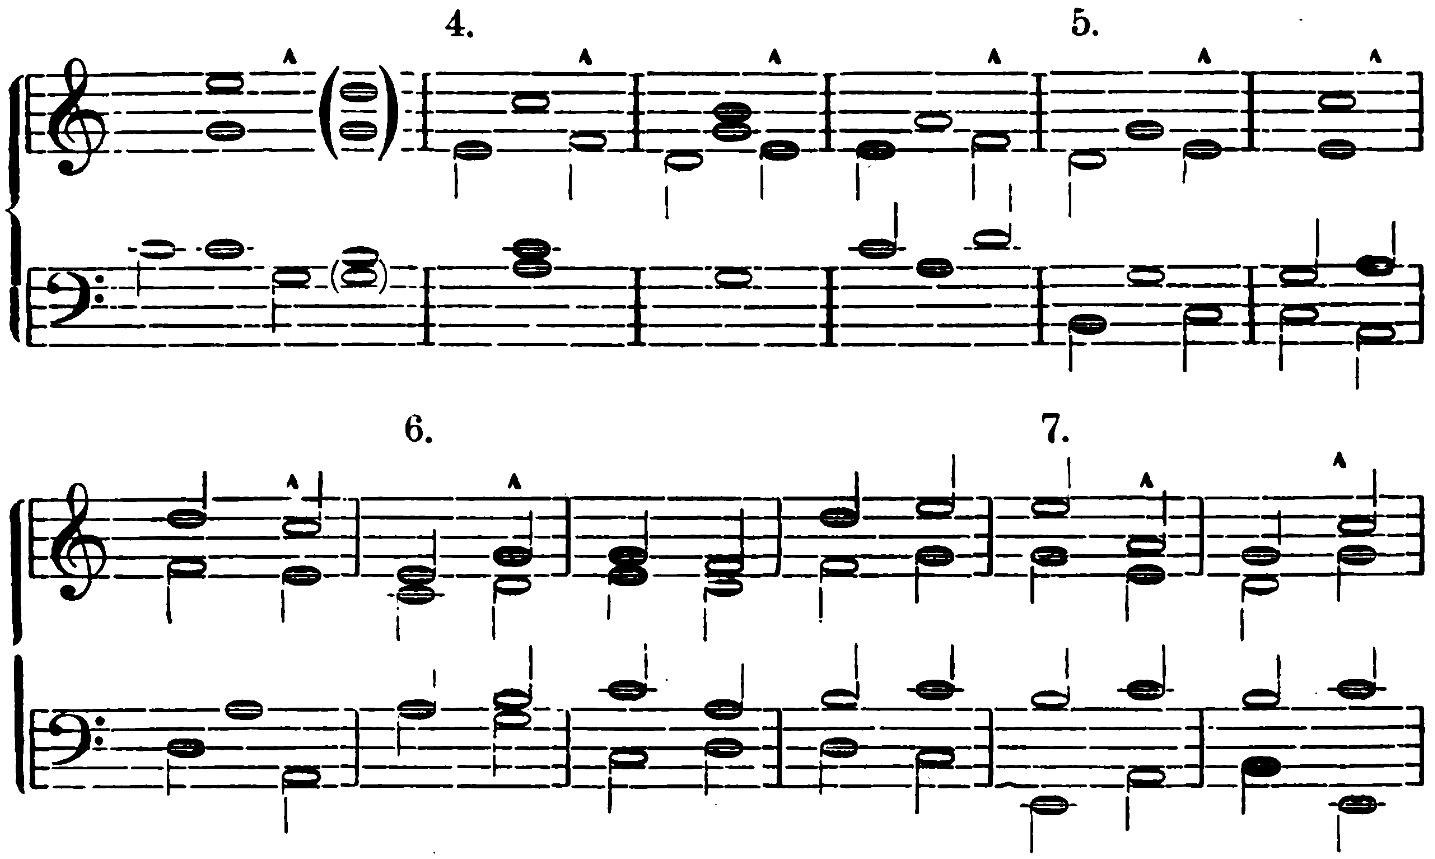
\includegraphics[width=.75\linewidth]{c/4/ex/mathias_graduated_2.png}\\
  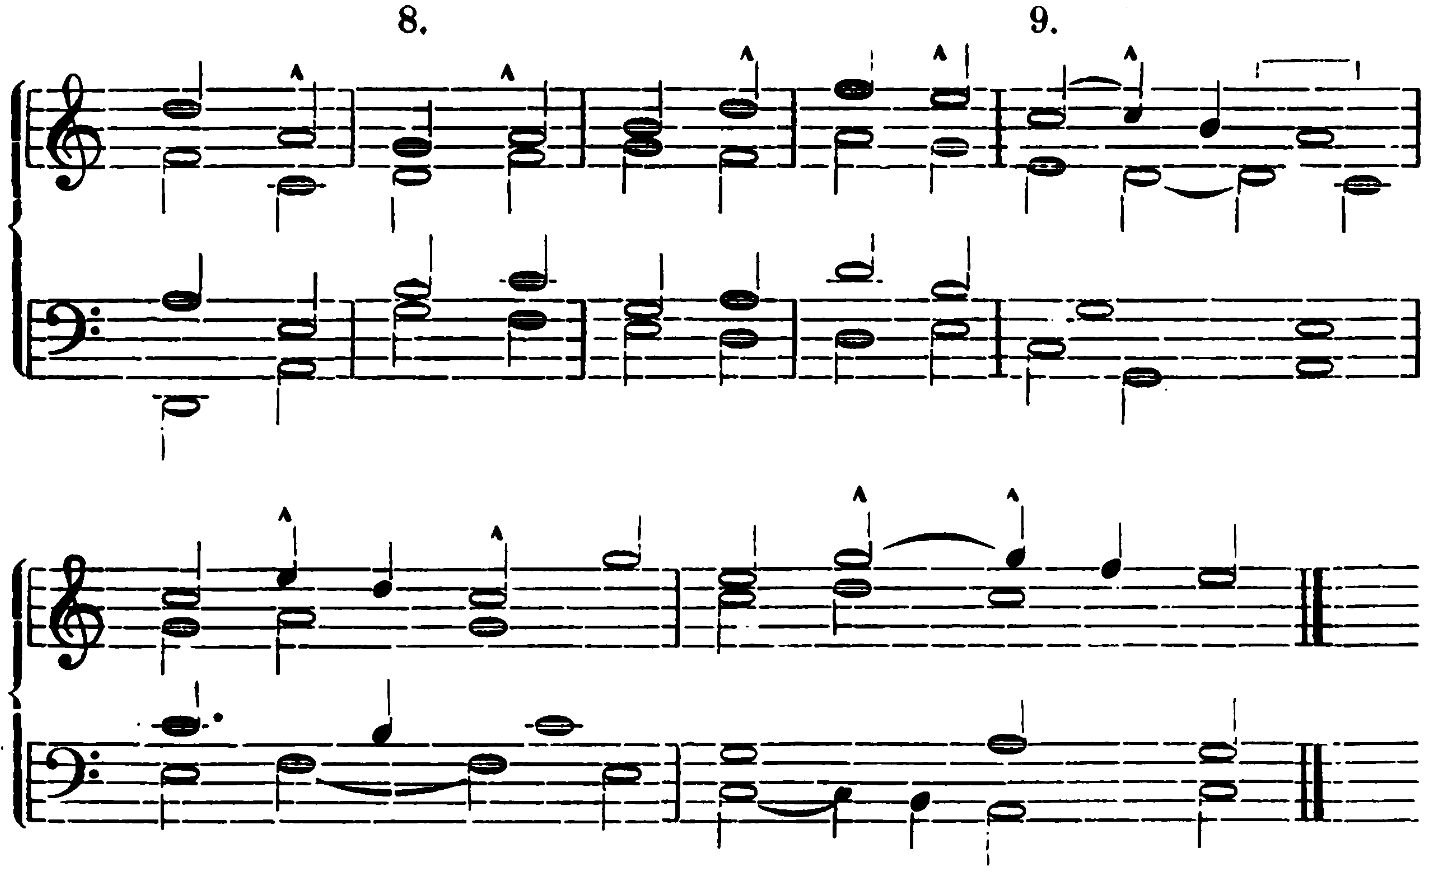
\includegraphics[width=.75\linewidth]{c/4/ex/mathias_graduated_3.png}\\
  \caption{Mathias, Graduated stages of part movement, 1903}
  \label{mus:mathias_graduated}
\end{example}

\vspace*{\fill}

\newpage

\vspace*{\fill}

\begin{example}
  \centering
  \includegraphics[width=.8\linewidth]{c/4/ex/mathias_messvesper_16.png}
  \caption{Mathias, Application of graduated stages}
  \label{mus:mathias_gratias}
\end{example}

\vspace*{\fill}


\begin{example}
  \centering
  \includegraphics[width=.8\linewidth]{c/4/ex/chassang_dissonances.jpg}
  \caption{Chassang, Dissonances marking \emph{ictus}, 1904}
  \label{mus:chassang_dissonances}
\end{example}

\vspace*{\fill}

\begin{landscape}

  \vspace*{\fill}

  \begin{example}
    \centering
    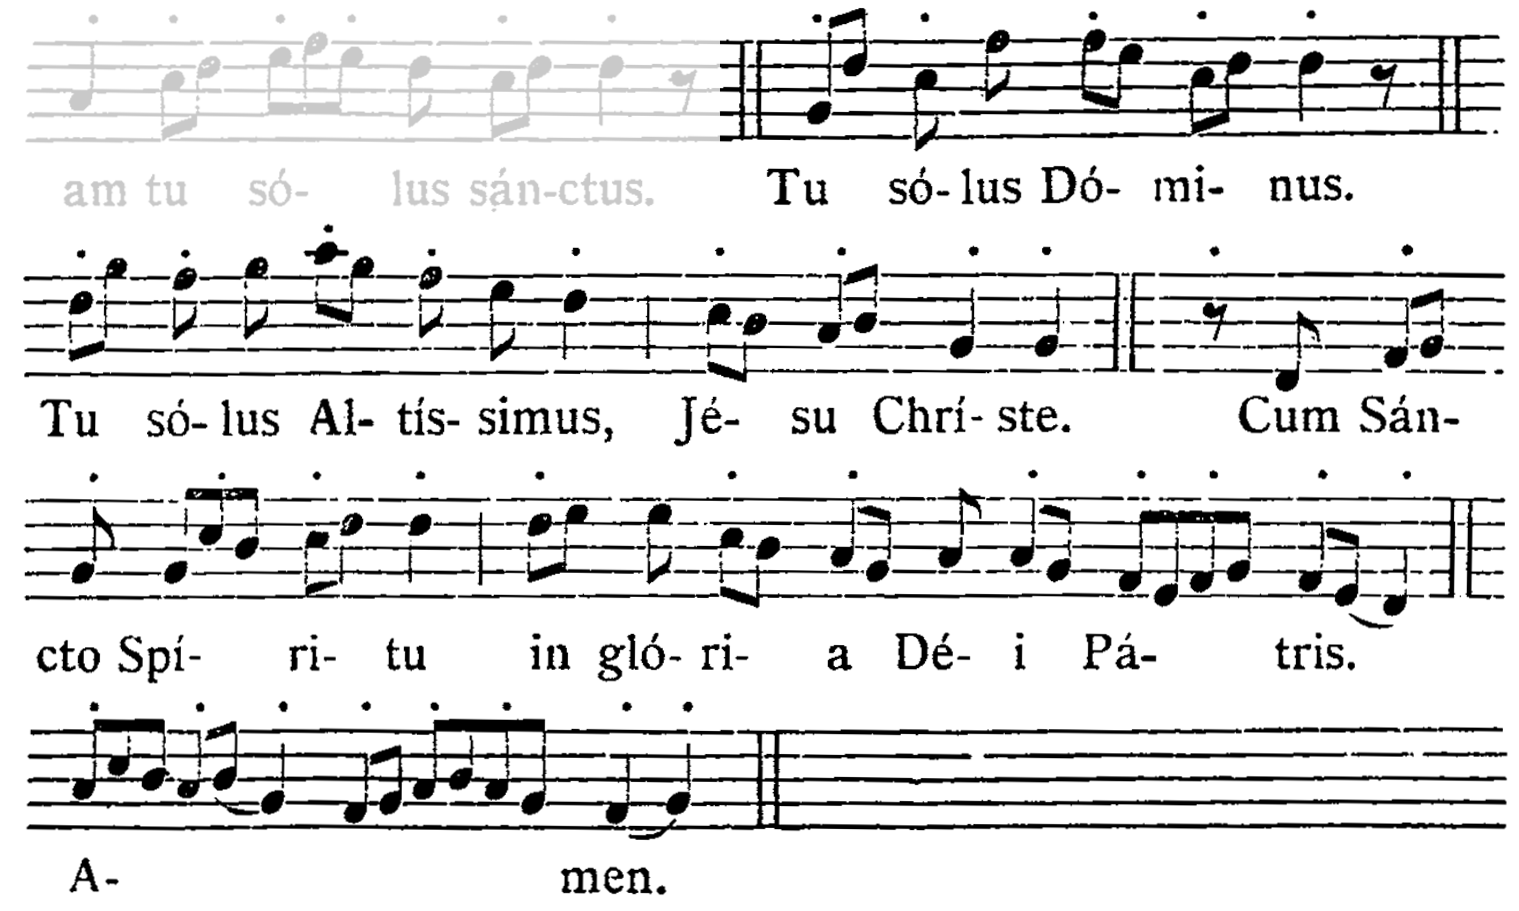
\includegraphics[width=.5\linewidth]{c/4/ex/moc_gloria_bonitatis.png}
    \caption{Mocquereau, Pointed `Gloria', 1904 (G2 clefs omitted)}
    \label{mus:moc_gloria_bonitatis}
  \end{example}

  \vspace*{\fill}

\end{landscape}



\begin{landscape}

  \vspace*{\fill}

  \begin{example}
    \centering
    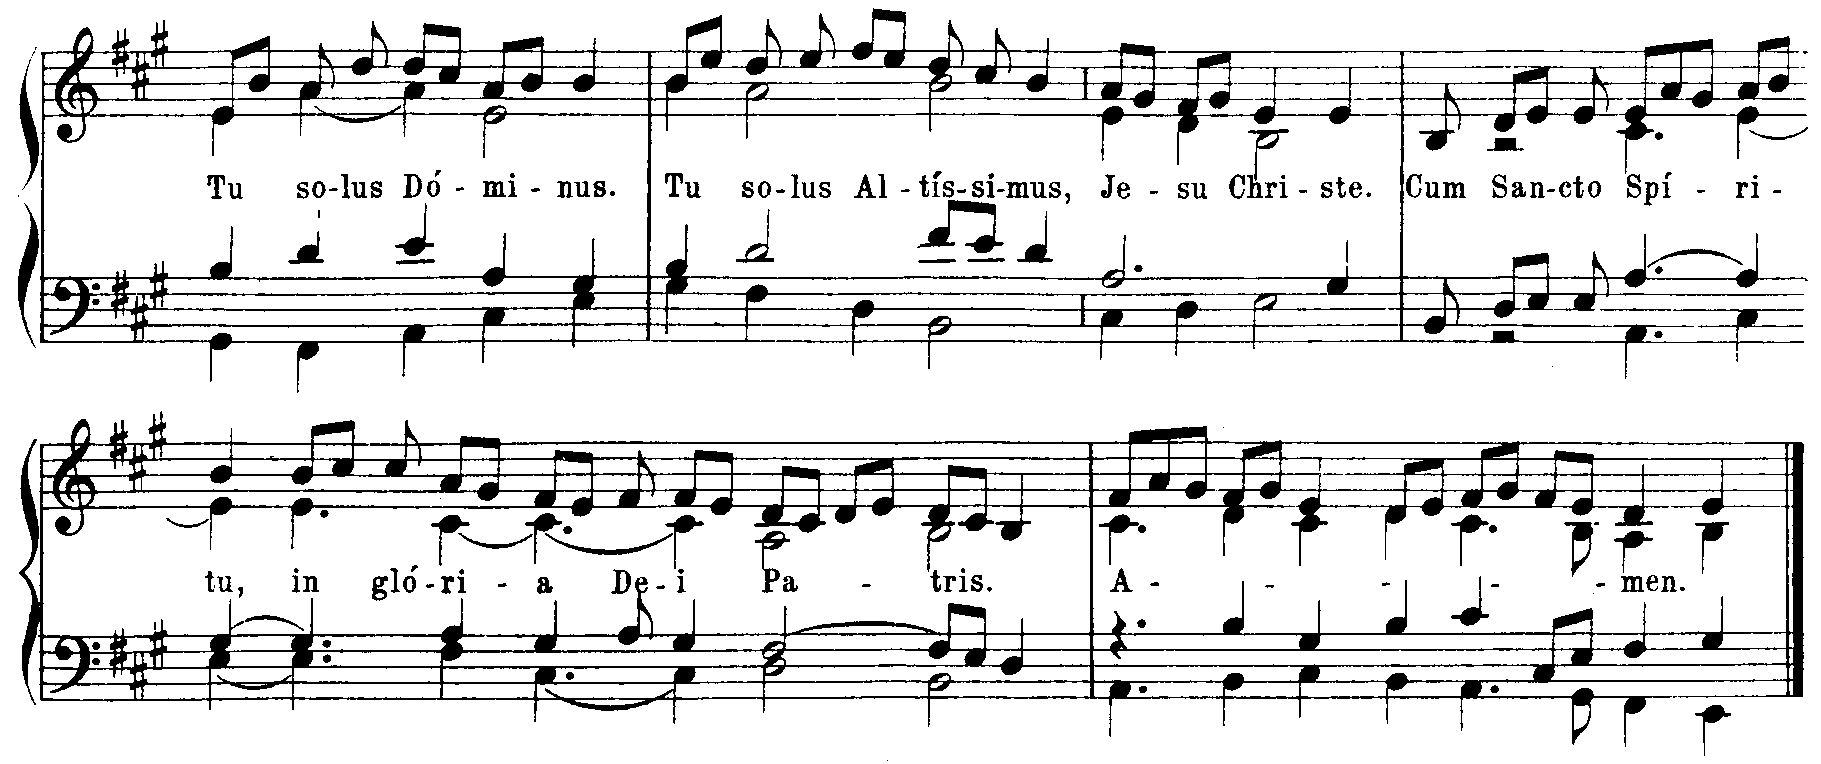
\includegraphics[width=.7\linewidth]{c/4/ex/mathias_moc.png}
    \caption{Mathias, Transcription similar to \cref{mus:moc_gloria_bonitatis}, 1905}
    \label{mus:mathias_moc_39}
  \end{example}

  \vspace*{\fill}

\end{landscape}

\begin{landscape}

  \vspace*{\fill}

  \begin{example}
    \centering
    \includegraphics[width=.7\linewidth]{c/4/ex/wagner_jubilo_42.png}
    \caption{Wagner, Flitting between two, three and four parts, 1905}
    \label{mus:wagner_jubilo_42}
  \end{example}

  \vspace*{\fill}




  \begin{example}
    \centering
    \includegraphics[width=.6\linewidth]{c/4/ex/desmetdupuydt_notation_97.png}
    \caption{Desmet--Dupuydt, Filled-and-void notation, 1910s}
    \label{mus:desmetdupuydt_notation_97}
  \end{example}

  \vspace*{\fill}

\end{landscape}

\begin{landscape}

  \vspace*{\fill}

  \begin{example}
    \centering
    \includegraphics[width=.7\linewidth]{c/4/ex/horn_kyriale_1.png}
    \caption{Horn, \emph{Quilisma} and caret symbols, 1932}
    \label{mus:horn_kyriale_1}
  \end{example}

  \vspace*{\fill}

  \begin{example}
    \centering
    \includegraphics[width=.8\linewidth]{c/4/ex/bas_angelis_repertorio_15.JPG}
    \caption{Bas, Double signatures, 1904}
    \label{mus:bas_angelis_repertorio_15}
  \end{example}

  \vspace*{\fill}

\end{landscape}

\begin{landscape}

  \vspace*{\fill}

  \begin{example}
    \centering
    \includegraphics[width=.8\linewidth]{c/4/ex/mathias_transposition_44.png}
    \caption{Mathias, Double signatures, 1906}
    \label{mus:mathias_transposition_44}
  \end{example}

  \vspace*{\fill}

  \begin{example}
    \centering
    \includegraphics[width=.8\linewidth]{c/4/ex/nekes_sharps.jpg}
    \caption{Nekes, Deuterus cadences with sharps}
    \label{mus:nekes_sharps}
  \end{example}

  \vspace*{\fill}

\end{landscape}

\begin{landscape}

  \vspace*{\fill}

  \begin{example}
    \centering
    \includegraphics[width=.9\linewidth]{c/4/ex/johanns_50.png}
    \caption{Johanns, Cadential sharping, 1909}
    \label{mus:johanns_50}
  \end{example}

  \vspace*{\fill}

\end{landscape}

\vspace*{\fill}

\begin{example}
  \centering
  \includegraphics[width=.8\linewidth]{c/4/ex/solesmes_vatican_28star.png}
  \caption{Solesmes, Updated chant to match Vatican Edition, 1905}
  \label{mus:solesmes_vatican_28star}
\end{example}

\vspace*{\fill}

\begin{example}
  \centering
  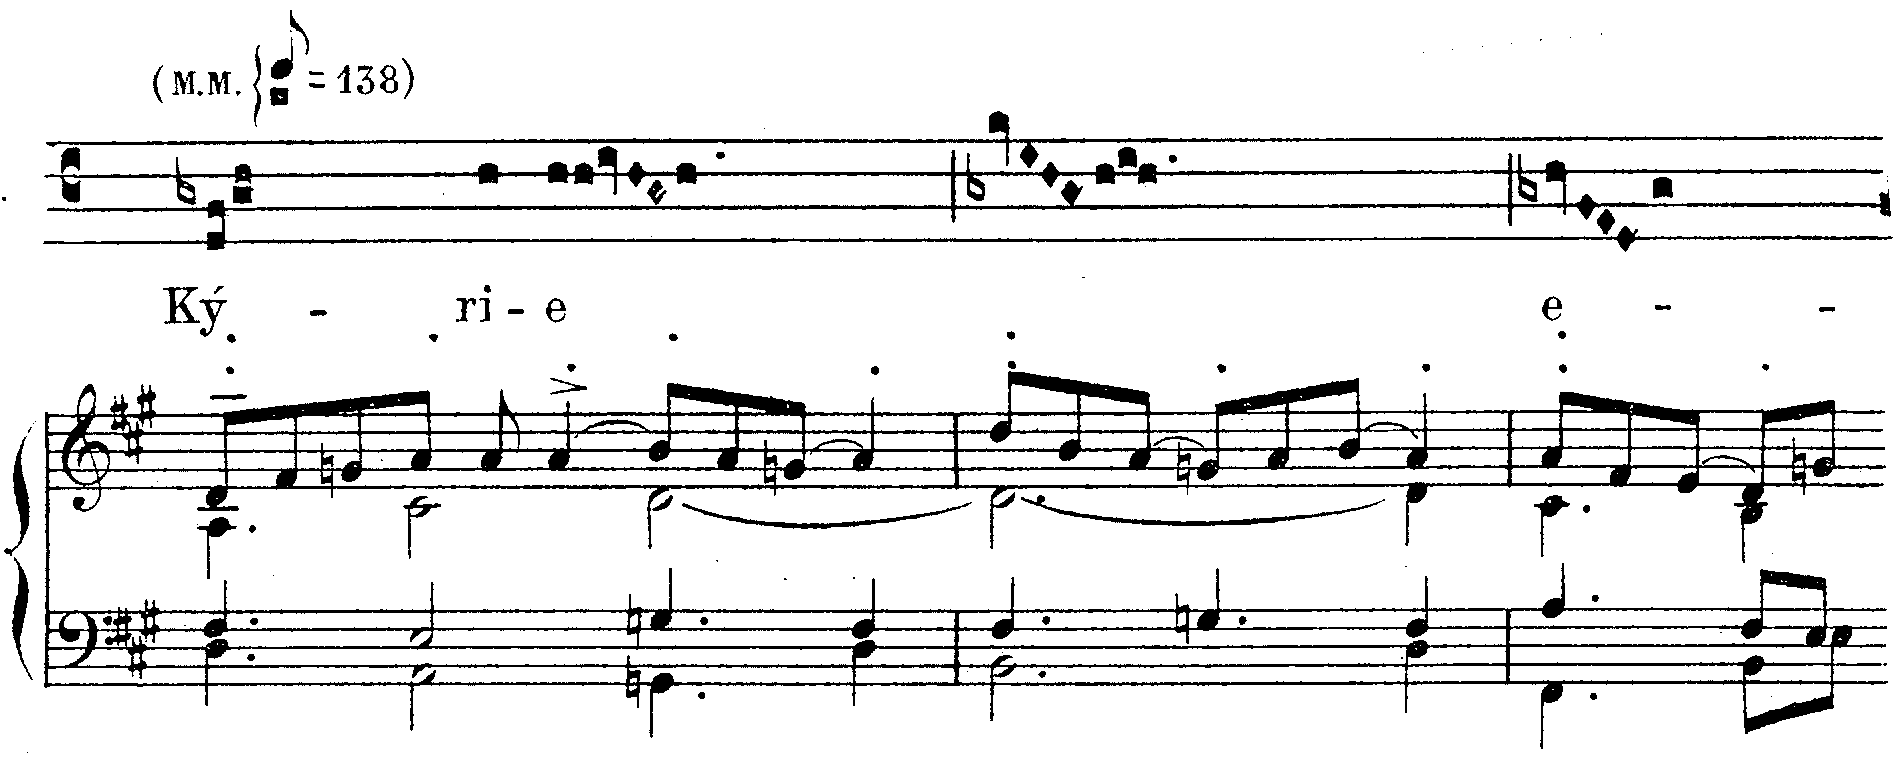
\includegraphics[width=\linewidth]{c/4/ex/delpech_angelis_34.png}
  \caption{Delpech, Chord placement matches pointing, 1898}
  \label{mus:delpech_angelis_34}
\end{example}

\vspace*{\fill}

\begin{landscape}

  \vspace*{\fill}

  \begin{example}
    \centering
    \includegraphics[width=.8\linewidth]{c/4/ex/bas_angelis_kyriale_40.png}
    \caption{Bas, Revised accompaniment, 1906}
    \label{mus:bas_angelis_kyriale_40}
  \end{example}

  \vspace*{\fill}

\end{landscape}

\begin{landscape}

  \vspace*{\fill}

  \begin{example}
    \centering
    \includegraphics[width=.5\linewidth]{c/4/ex/solesmes_liber_1924_39.png}
    \caption{Solemses, Pointing with vertical \emph{episemata}, 1924}
    \label{mus:solesmes_liber_1924_39}
  \end{example}

  \vspace*{\fill}

\end{landscape}

\begin{landscape}

  \vspace*{\fill}

  \begin{example}
    \centering
    \includegraphics[width=\linewidth]{c/4/ex/manzetti_angelis_48.png}
    \caption{Manzetti, Reportedly following Bas, 1906}
    \label{mus:manzetti_angelis_48}
  \end{example}

  \vspace*{\fill}

\end{landscape}

\vspace*{\fill}

\begin{example}
  \centering
  \includegraphics[width=\linewidth]{c/4/ex/mathias_secondary_89.png}
  \caption{Mathias, Secondary accidental pertains to chant part alone, 1936}
  \label{mus:mathias_secondary_89}
\end{example}

\vspace*{\fill}

\begin{example}
  \centering
  \includegraphics[width=\linewidth]{c/4/ex/wiltberger_deuterus_60.png}
  \caption{Wiltberger, Sharped deuterus cadence, \emph{c}.1910}
  \label{mus:wiltberger_deuterus_60}
\end{example}

\vspace*{\fill}

\begin{landscape}

  \vspace*{\fill}

  \begin{example}
    \centering
    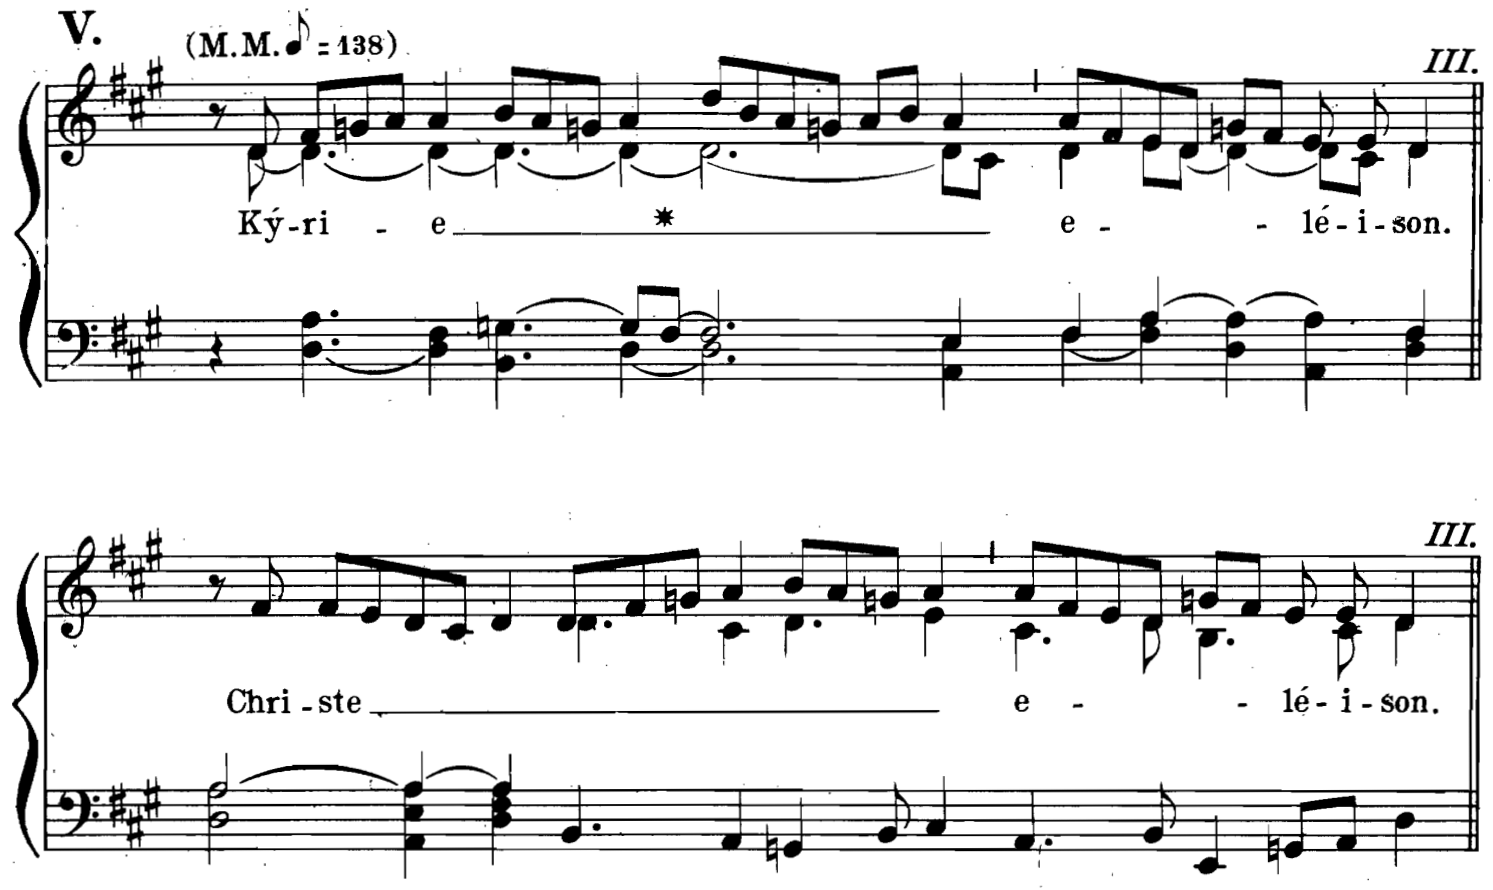
\includegraphics[width=.7\linewidth]{c/4/ex/vranken_angelis_7.png}
    \caption{Vranken, Seemingly following Solesmian transcription, 1910}
    \label{mus:vranken_angelis_7}
  \end{example}

  \vspace*{\fill}

\end{landscape}

\begin{landscape}

  \vspace*{\fill}

  \begin{example}
    \centering
    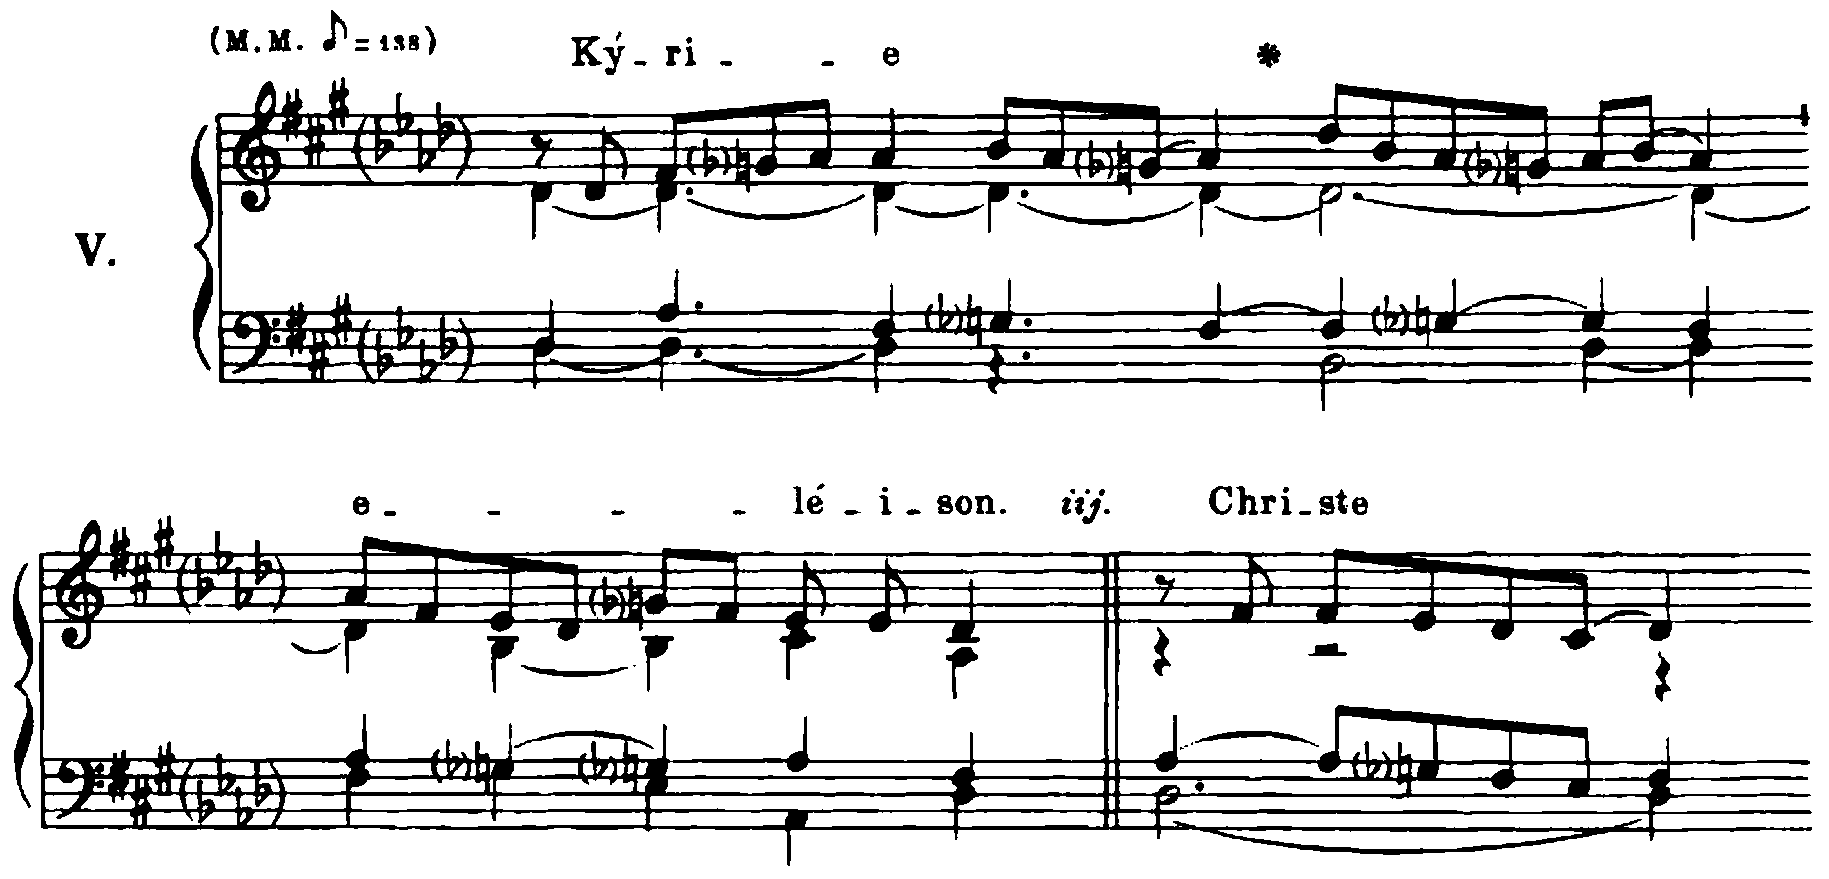
\includegraphics[width=.7\linewidth]{c/4/ex/boileau_angelis_1.png}
    \caption{Benedictonos de Besalú Girona, \emph{Ibid}.}
    \label{mus:boileau_angelis_15}
  \end{example}

  \vspace*{\fill}

\end{landscape}

\vspace*{\fill}

\begin{example}
  \centering
  \includegraphics[width=\linewidth]{c/4/ex/sablayrolles_parts.png}
  \caption{Sablayrolles, Number of parts determined by structure, 1912}
  \label{mus:sablayrolles_parts}
\end{example}

\vspace*{\fill}

\begin{example}
  \centering
  \includegraphics[width=\linewidth]{c/4/ex/foerster_asperges_17.png}
  \caption{Foerster, Rhythmed transcription, \emph{c}.1910}
  \label{mus:foerster_asperges_17}
\end{example}

\vspace*{\fill}

\begin{example}
  \centering
  \includegraphics[width=\linewidth]{c/4/ex/kimovec_angelis.png}
  \caption{Kimovec, Premrl showing supposed consecutives, 1908}
  \label{mus:kimovec_angelis}
\end{example}

\vspace*{\fill}

\newpage

\vspace*{\fill}

\begin{example}
  \centering
  \includegraphics[width=\linewidth]{c/4/ex/kimovec_communio_7.png}
  \caption{Kimovec, Chant notes harmonised as dissonances, 1909}
  \label{mus:kimovec_communio_7}
\end{example}

\vspace*{\fill}

\begin{example}
  \centering
  \includegraphics[width=\linewidth]{c/4/ex/kimovec_sharp_34.png}
  \caption{Kimovec, Anticipating `B'\kern 1pt\natural{}, 1909}
  \label{mus:kimovec_sharp_34}
\end{example}

\vspace*{\fill}

\begin{example}
  \centering
  \includegraphics[width=\linewidth]{c/4/ex/premrl_imitate_14.png}
  \caption{Kimovec, Imitative bass part, 1909}
  \label{mus:premrl_imitate_14}
\end{example}

\vspace*{\fill}

\newpage
